\section{Risk assessment for the DEMO++ gas system}

This section describes the riks assessment related with the operation of the DEMO++ gas system in the proposed experimental area (R015).

\subsection{Characteristics of the area}

The location of the experimental area can be seen in Fig. \ref{fig:location}. The size and distribution of the area can be seen in \ref{fig:Distribution2}. The area has a total surface of 25$m^2$, and a general view of the area is presented in Fig. \ref{fig:pictures}.

As it can be seen in Figure \ref{fig:Distribution2} and the area's pictures (Figure \ref{fig:pictures}) three of the walls and the floor appear to be reasonably gas tight. The area is open in one side, only covered with a metallic gate. Therefore we assume that any xenon gas leak will eventually diffuse though that gate.  

\begin{figure}
\centering
%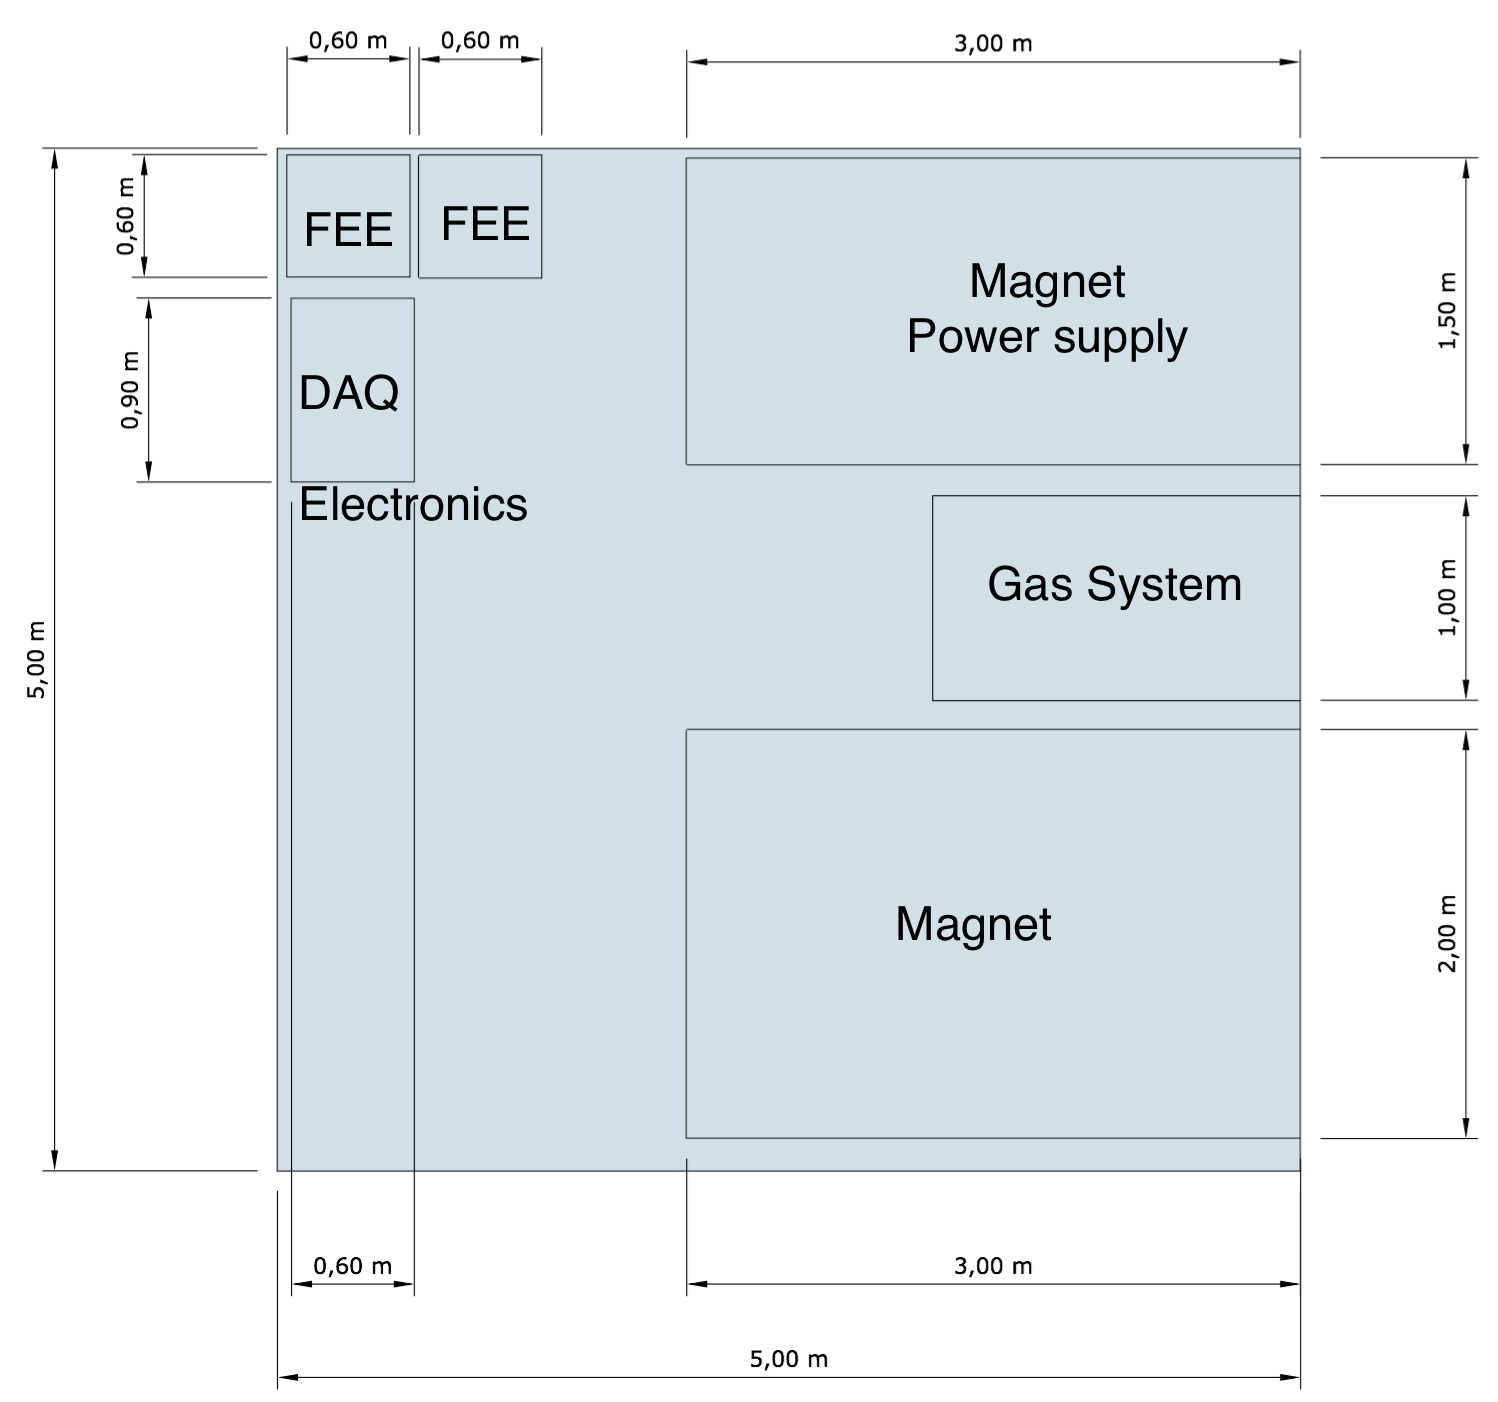
\includegraphics[width=\textwidth]{img/distribution2.png}
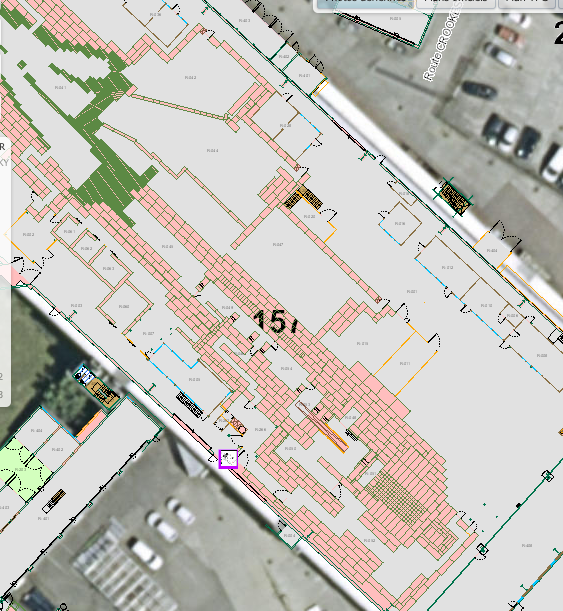
\includegraphics[angle=0,width=\textwidth]{img/generalmap.png}
\caption{Location of the experimental area} \label{fig:location}
\end{figure}


\begin{figure}
\centering
%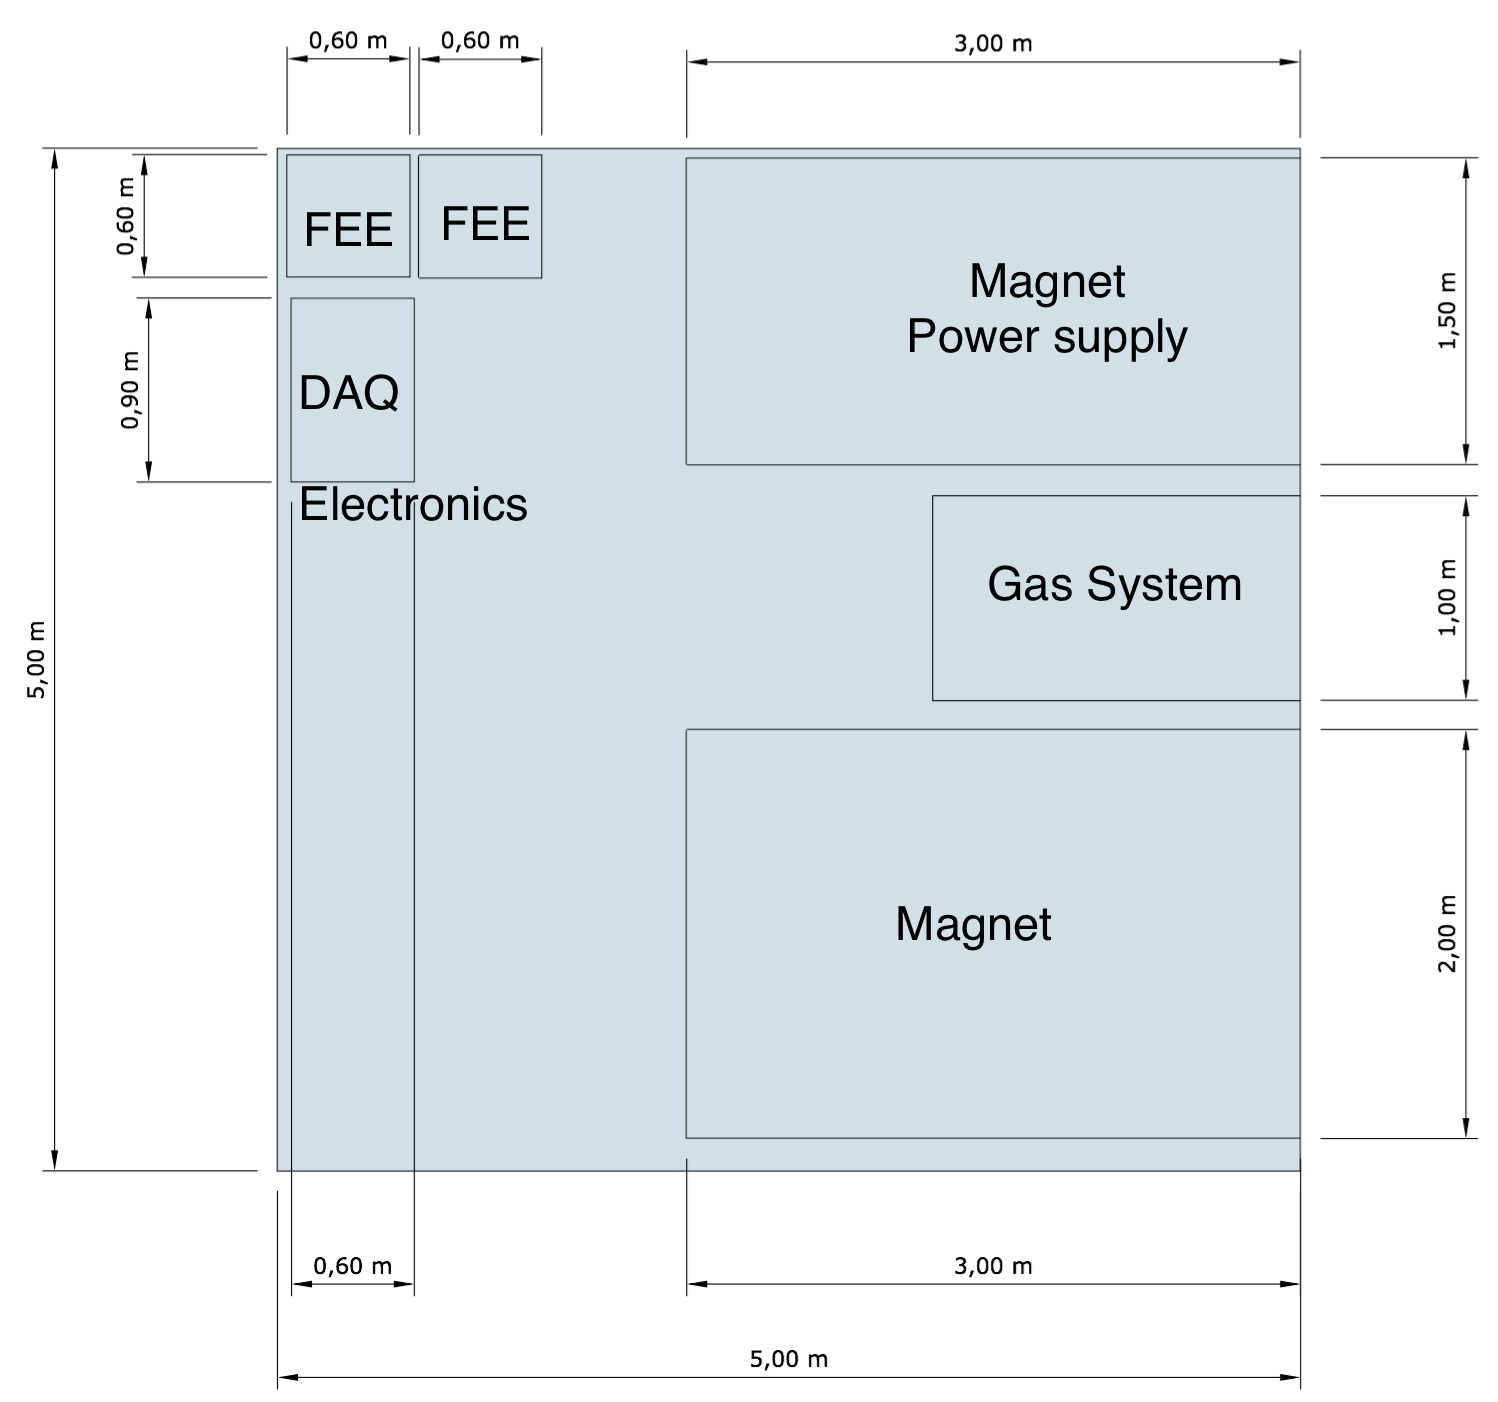
\includegraphics[width=\textwidth]{img/distribution2.png}
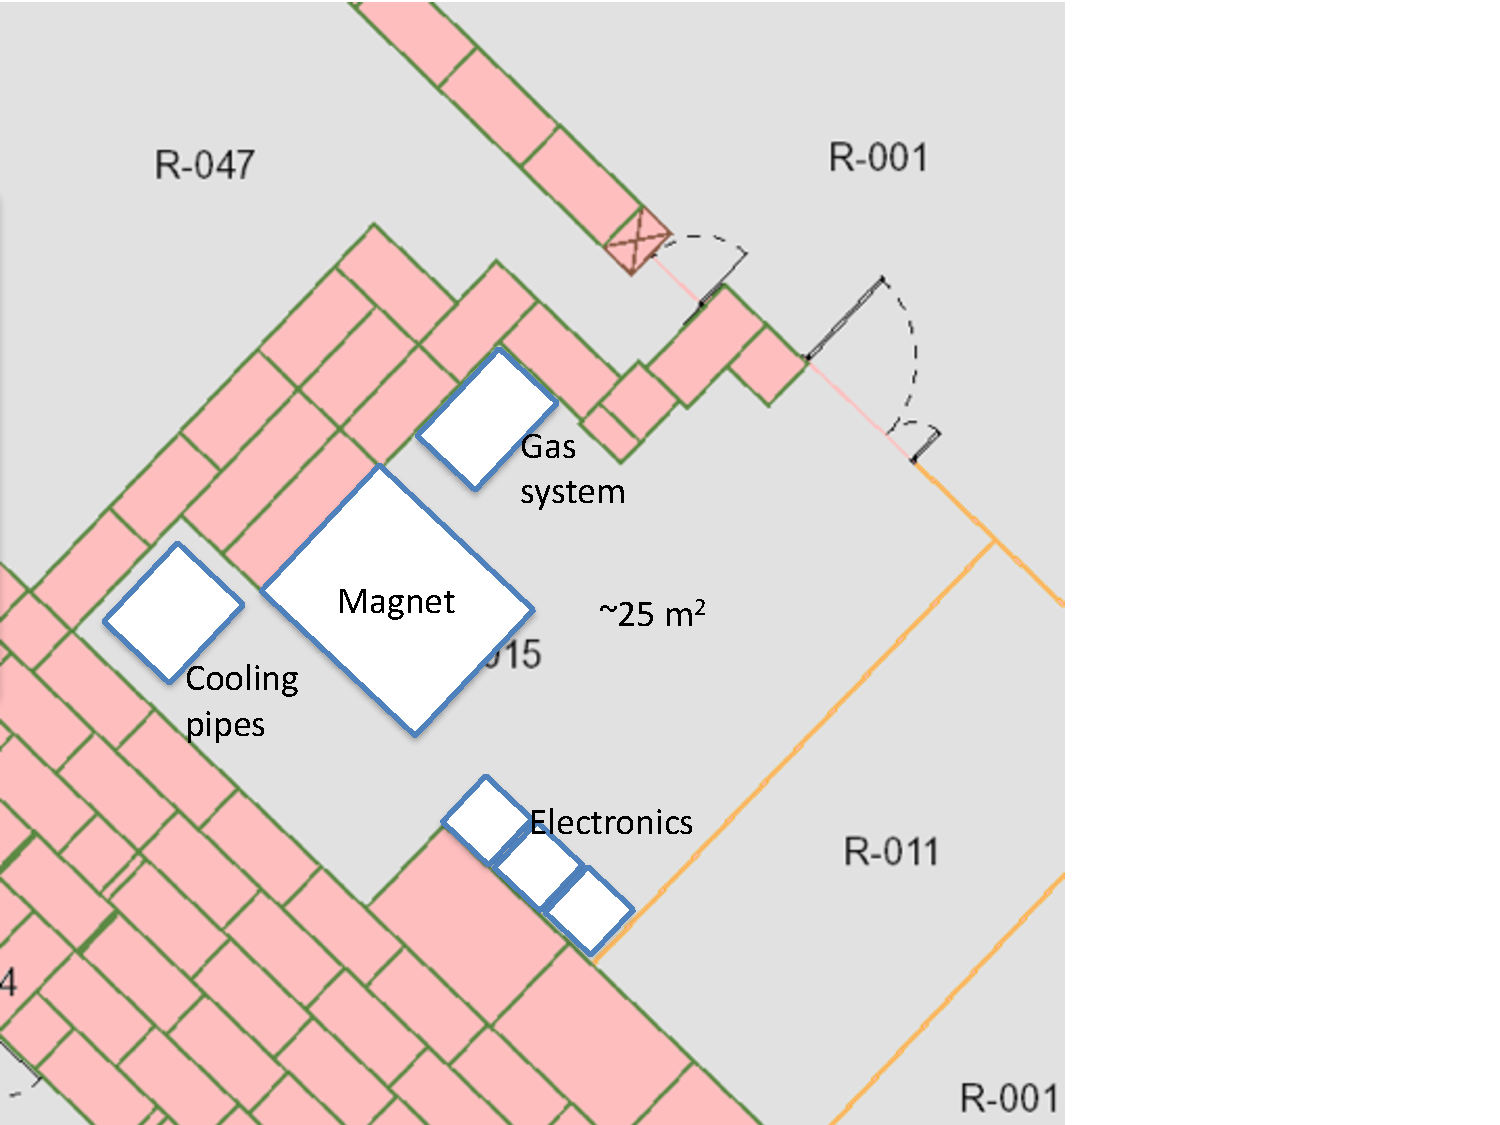
\includegraphics[angle=0,width=\textwidth]{img/distribution_examples.pdf}
\caption{Proposed distribution of the NEXT-DEMO, magnet and all different necessary systems for the operation of the detector in the experimental area} \label{fig:Distribution2}
\end{figure}


\begin{figure}
\centering
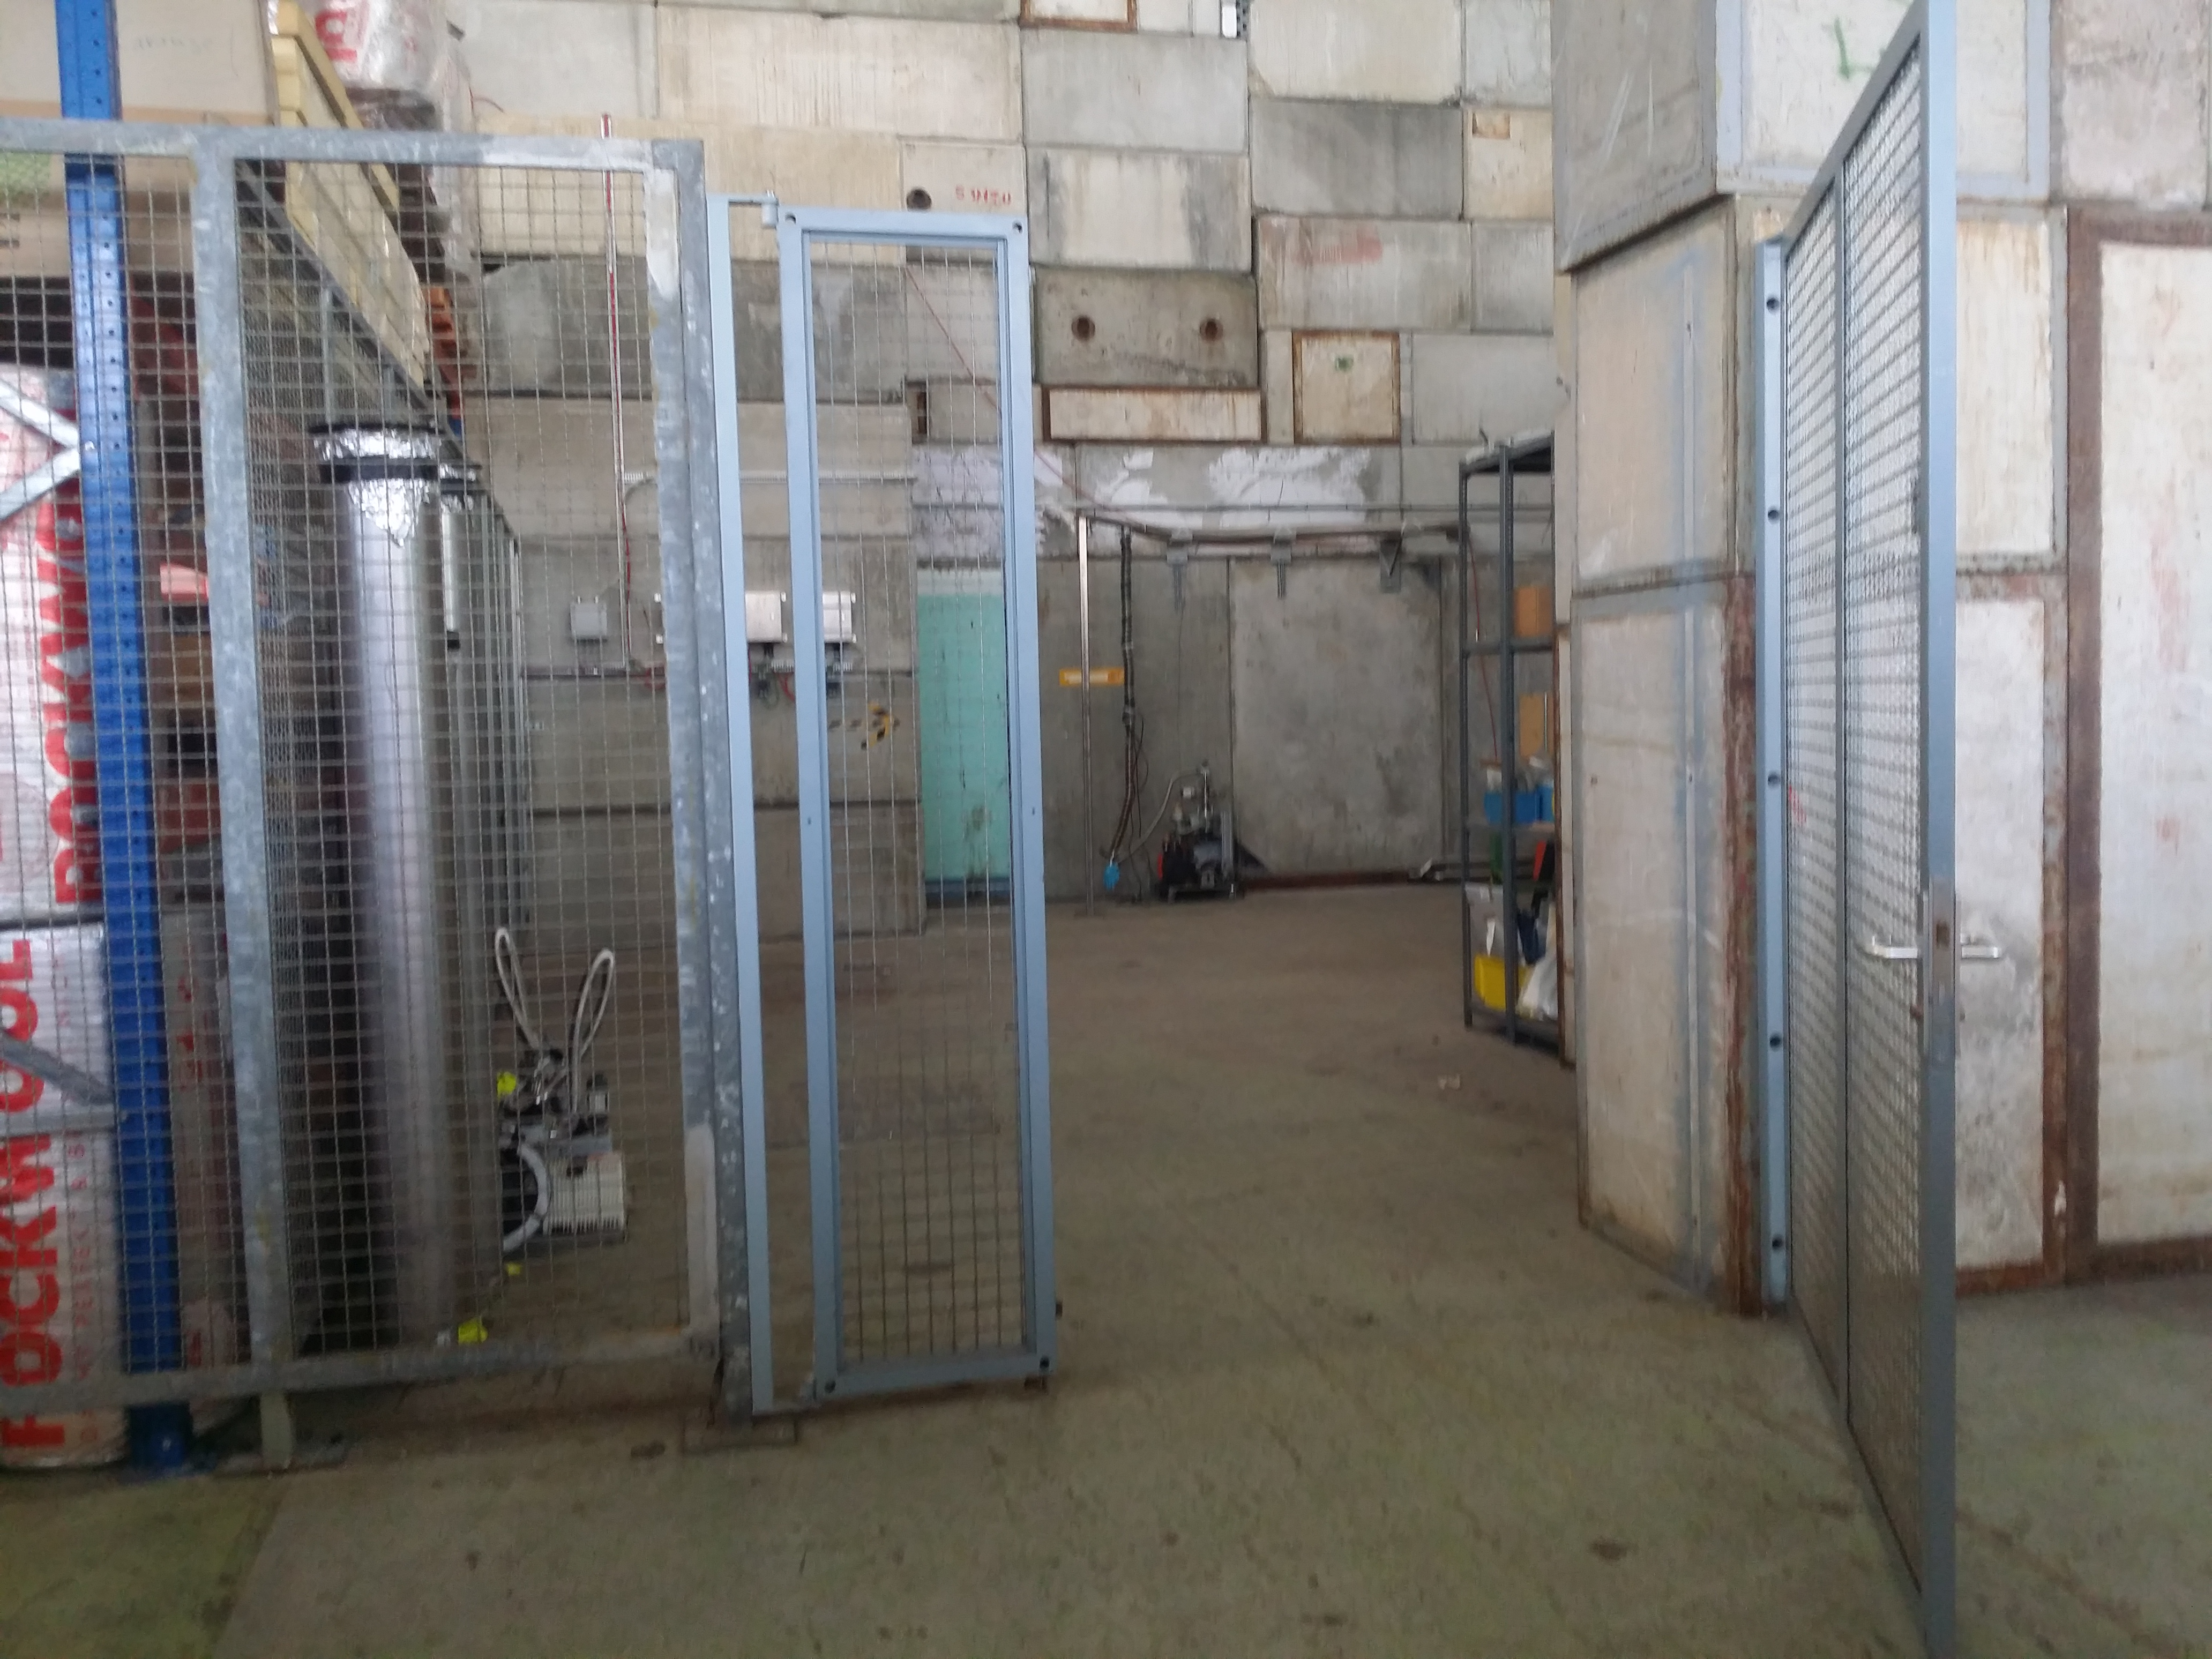
\includegraphics[width=0.45\textwidth]{img/experimentalarea1.jpeg}
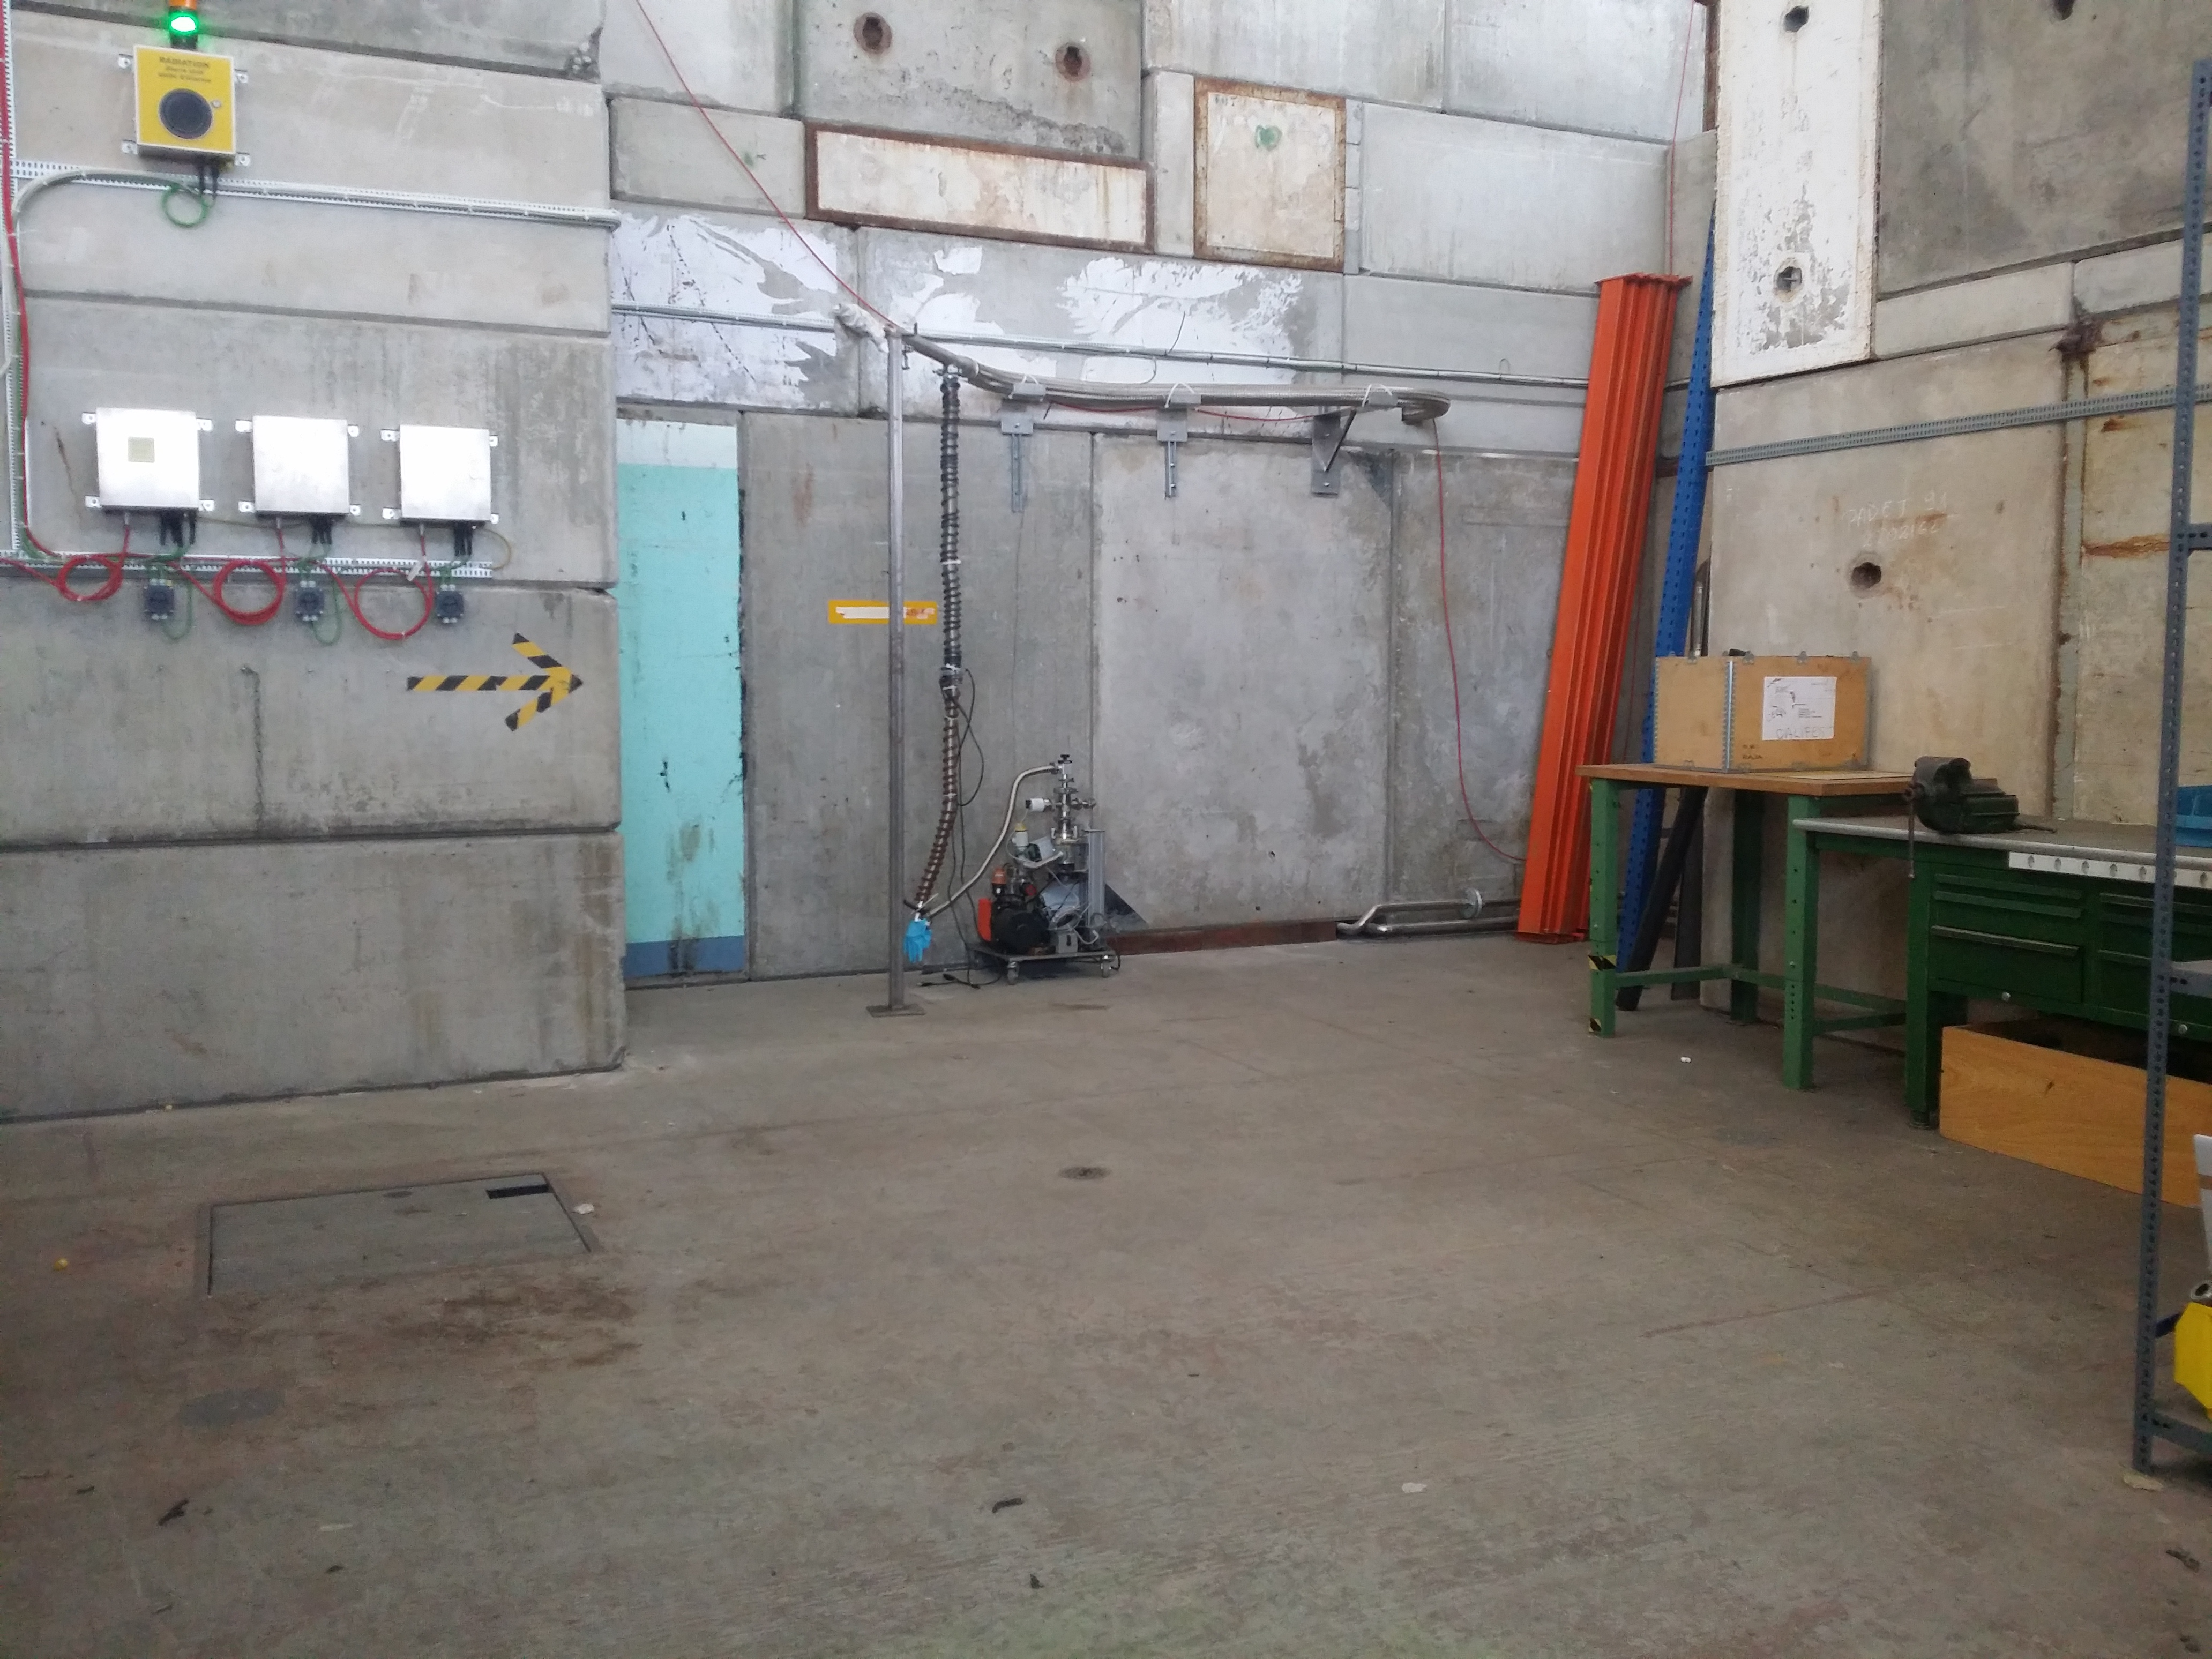
\includegraphics[angle=0,width=0.45\textwidth]{img/experimentalarea2.jpeg}
\caption{Proposed distribution of the NEXT-DEMO, magnet and all different necessary systems for the operation of the detector in the experimental area} \label{fig:pictures}
\end{figure}


\subsection{Related Gas systems}

Only one gas system will be used in the area. The gas system has been described in the main document. We recall that the amount of CO$_2$~needed is only of the order of 0.5 \% max, therefore, 5 grams for a xenon load of 1 kg (which is the operational load of DEMO++). Such small amount of gas only requires a bottle of 25 grams. We assume, however, a larger bottle of 100 grams which may be easier to handle. The following table summarizes the quantity and distribution of the different gases to be used in NEXT-DEMO:



\begin{table}[h]
%\resizebox{1.4\textwidth}{!}{\begin{minipage}{\textwidth}
\begin{tabular}{|r|r|r|r|r|}
\hline
\parbox[t]{2cm}{Gas Type} & \parbox[t]{3cm}{Supply description} & \parbox[t]{2cm}{Mass} &\parbox[t]{3cm}{ Volume (gas at ambient P ad T) }& \parbox[t]{3cm}{Supply location (see figure \ref{fig:Distribution2}) }\\\hline
Xenon & One bottle & 1500 g & 255 liters & GS 1  \\\hline
CO2 & One bottle & 100 g & 50 liters (approx.) & GS 1 \\\hline
\end{tabular}
\caption{Gas supply for NEXT-DEMO}
\label{tab:gassupply}
%\end{minipage} }
\end{table}

\subsection{Gas release risk assesment}

\subsubsection{Relevant Facts}
\begin{itemize}
\item All gases are at room temperature during normal operation.
\item A gas leak of the order of 1\% is easily detected.
\item All used gases are transparent and odorless.
\item All used gases are non-flamable. 
\end{itemize}

\subsubsection{Risk assesment}

\textit{Scenario 1}

A leak due to a crack in the gas system or the compressor, or due to an accidental impact that causes a hole in the system. The worst case scenario assumes that one of the pipes or flexible connection breaks. The largest pipes/flexibles in the system have a diameter of 1/2''. The result of such an event is a total, and very fast, loss of the gas.  

\textbf{Consequences:} In the above scenario, the gas is released at a flow of 2060 litres per minute, therefore, the total volume escapes in a few seconds. The slow control will detect the pressure dropped and take the following actions:
\begin{enumerate}
\item Stop the compressor.
\item Ramp down all the voltages. 
\item Activate an alarm in the experimental area. One could consider to include a second alarm in the underground galleries, although the risk appears to be negligible (see discussion below). 
\item Send electronic notification of failure to remote control systems.
\end{enumerate}

The associated hazard is the risk of asphyxiation due to the air being displaced by the released gas. Given that the area is open, the volume of CO$_2$ mould mix up in the air and would not posses any significant hazard. Xenon does not mix with air and tends to drop to floor level due to its weight. Since the area is open, xenon will also eventually diffused out of the area. 

To give an estimation of the worst case scenario we consider the case in which the area is assumed to be gas tight. In this case, the released volume (255 l) would occupy a surface of 25 m$^2$ and reach a height of 10.2 cm, which corresponds to the ankle of a normal height person. Since the area, far from being tight is fully open in one side, the gas will expand in a much larger area and pose no threat. 

A possible residual hazard would be that xenon leaks into the underground gallery of the power cables. However, the total volume is small, and will, again, diffuse very quickly. Nonetheless we propose to install an oxygen monitor in the area and another one in the entrance of the power cable gallery. Should those monitors (which will be connected to slow controls) detect any significant drop in the amount of oxygen, an alarm will be fired. 


\textit{Scenario 2}
 
 A leak occurs during cryogenic recovery of the Xenon. 
 
 \textbf{Consequences:} In this case the slow control will not respond to a drop of pressure. On the other hand, most of the Xenon should be frozen and the total volume of Xenon released to the atmosphere will be very small compared with the case previously considered. In any case, the presence of the oxygen monitors will guarantee safe operation. 
 

\subsection{Conclusions}

\subsubsection{Oxygen detection hazard}

It appears that CO$_2$~poses no risk whatsoever. The hazard associated with xenon release (asphyxiation) seems to be negligible even in the event of total and sudden release, given the fact that the experimental area is open and the total amount of gas is small. Nonetheless, we propose to install one Oxygen Detection Head (ODH) in the experimental area, and another one in the underground gallery connecting through which the power cables arrive. 

We propose the installation of three alarms (flashing red light and a a noise signal). One inside the experimental area, another one in the external part of the area, near the door and a third one in the underground gallery. 
